


En esta parte abarcaremos qué es un robot, la posible equivalencia entre robot y autómata y la evolución de estos conceptos a lo largo del tiempo. Es decir, claro queda que un robot debe ser un tipo de máquina, pero la noción de lo que es una máquina ha variado significativamente a lo largo del tiempo. 

\vspace{10px}

Nadie dudaría sobre la veracidad de la siguiente afirmación 'Un ordenador es una máquina'; sin embargo, hay una diferencia cualitativa importante entre un ordenador y un actuador mecánico, por ejemplo: una puerta automática.

\vspace{10px}

La noción de automatismo será clave para discernir qué es o no es un robot. 

\vspace{10px}





\subsection{Conceptualización de la máquina y el autómata.}

Hemos hablado de lo complicado que resulta dar una definición completa de estos conceptos, pues aunque todos sepamos qué es una maquina por extensión, las cualidades que comparten los objetos que llamamos máquinas pueden llegar a ser muy escasas.

\subsubsection{Álgebras de Boole y sistemas combinacionales}

En el siglo XIX se da otro gran avance cualitativo sobre el entendimiento de qué cosas son máquinas, alejándonos de la definición clásica de los mecanicistas y entrando en el campo de la lógica.

\vspace{10px}

Las álgebras de Boole son la base teórica de los sistemas combinacionales (S.C.). Un sistema combinacional es una máquina (según hemos definido) cuya salida es únicamente función de su entrada, es decir, no presenta memoria sobre ningún estado pasado. Este será un aspecto fundamental en el avance de las 'máquinas', su memoria. La habilidad de poder tener presente situaciones anteriores para deliberar en la ejecución actual, y en qué medida se pueda hacer esto, marcará toda una escala de complejidad.

\vspace{10px}


La realización de este concepto se ve con gran claridad en los circuitos lógicos, a partir de operaciones simples ( como son la negación, la disyunción y la conjunción ) podemos llegar a expresar teóricamente cuál sería el funcionamiento de un sistema lo suficientemente complejo como para realizar operaciones artiméticas a mayor velocidad que un humano.

\vspace{10px}

Queremos destacar que aunque estos sistemas se consideran típicamente como digitales, hechos a base de transistores recibiendo impulsos eléctricos, no tienen una diferencia cualitativa importante en cuanto a capacidad de computo o expresividad con un sistema mecánico clásico.

\vspace{10px}

En 1642 el filósofo y matemático francés Blaise Pascal inventó una calculadora mecánica, \textbf{La pascalina}. Aunque es evidente que hay una gran diferencia entre una calculadora mecánica y una digital, ambas pueden conceptualizarse como sistemas combinacionales; ya que ninguna de las dos tiene memoria sobre ejecuciones anteriores (estados) y el sistema, sean cuales sean sus actuadores, produce una salida como función única de una entrada. 


\subsection{Autómatas finitos}


En el siglo XX nace la teoría de autómatas como siguiente nivel de conceptualización sobre qué son las máquinas y qué pueden hacer, la pregunta fundamental de este momento histórico es: ¿Qué problemas puede resolver una máquina?.

\vspace{10px}

Daremos ahora una definición de autómata alejada del mecanicismo anterior, más parecido al modelo abstracto de las álgebras de Boole: Un autómata finito es una máquina (abstracta) cuya salida no depende solo de la entrada actual.

\vspace{10px}

Un autómata finito tiene estados, posiciones de memoria que dependerán de las entradas anteriores, esto eleva la capacidad expresiva del autómata muy por encima de la del S.C. \\

- En electrónica un autómata es un sistema secuencial, aunque en ocasiones la palabra es utilizada también para referirse a un robot. [...] Sin embargo, la rápida evolución de los autómatas hace que esta definición no esté cerrada. (Wikipedia)- \\

Aquí un sistema secuencial es justo lo que hemos definido como autómata, un sistema combinacional dotado de memoria.  Un ejemplo muy sencillo de un cálculo que podría hacerse con un autómata finito y no bastaría con un sistema combinacional, sería la tarea de decidir si un conjunto de ceros es par o impar. Esto puede parecer una tarea trivial pero es un cálculo recurrente en la comprobación de errores de protocolos de comunicación tan conocidos como el TCP/IP, que implementan un bit de paridad para este fin.

\vspace{10px}


Definiremos qué es un autómata con más rigurosidad en lo que sigue, pero por ahora, daremos un ejemplo de lo que será un autómata bajo el formalismo que plantearemos. El robot WATBOT1 tenía una interfaz conversacional implementada, pues bien, dicha interfaz se modelaba mediante un autómata finito. Es decir: El robot en sí no era el autómata, el mecanismo que le permitía dialogar (aunque fuese de manera precaria) se modeló con una máquina de estado finito.

\subsubsection{Aumentando la abstracción: Lenguajes y problemas }


Esta evolución sobre lo que era una máquina y qué problemas podía resolver planteó el mismo problema que habíamos subrayado antes. Si podemos clasificar las máquinas que tenemos según su complejidad, ¿podríamos hacerlo con los problemas?

\vspace{10px}

Este es fundamentalmente el objeto de estudio de la teoría de autómatas, pues responde fundamentalmente a la pregunta: ¿Qué máquina necesito para resolver este problema?

\vspace{10px}

La definición del lenguaje formal como se hace en esta teoría es bastante natural:

\vspace{10px}


Sea  $\mathcal{A}$ un conjunto finito de símbolos, a este conjunto lo llamaremos alfabeto, muy en consonancia con el uso popular del concepto. A los símbolos de $\mathcal{A}$ se les llamará letras, a las secuencias finitas de letras, palabras, y a todas las palabras que se puedan formar con las letras se las conoce como lenguaje generado por $\mathcal{A}$ o por sintetizar: $\mathcal{A}^{*}$. Un lenguaje sobre $\mathcal{A}$, será un subconjunto de su lenguaje generado. Esto es:


$$ \mathcal{L} \text{ es un lenguaje sobre } \mathcal{A}  \iff \mathcal{L} \subset \mathcal{A^{*}} $$


Hasta aquí existe un paralelismo evidente con lo que asociaríamos con un lenguaje de manera popular. Pues bien, existe una relación entre las categorías de complejidad que mencionamos antes y los lenguajes. \\ 


Por ejemplo, definamos el siguiente lenguaje, palabras sobre $\{0,1\}$ tales que tengan un número par de 0's.

\begin{equation}
\mathcal{L} = \{\omega \in \{0,1\}^{*} : \text{ $\omega$ tiene un nº par de 0's} \}
\end{equation}


\begin{center}
	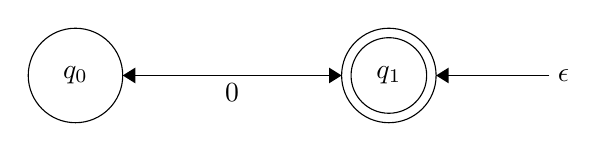
\begin{tikzpicture}[scale=0.2]
	\tikzstyle{every node}+=[inner sep=0pt]
	\draw [black] (40.6,-19.3) circle (3);
	\draw (40.6,-19.3) node {$q_1$};
	\draw [black] (40.6,-19.3) circle (2.4);
	\draw [black] (20.7,-19.3) circle (3);
	\draw (20.7,-19.3) node {$q_0$};
	\draw [black] (37.6,-19.3) -- (23.7,-19.3);
	\fill [black] (23.7,-19.3) -- (24.5,-19.8) -- (24.5,-18.8);
	\draw [black] (23.7,-19.3) -- (37.6,-19.3);
	\fill [black] (37.6,-19.3) -- (36.8,-18.8) -- (36.8,-19.8);
	\draw (30.65,-19.8) node [below] {$0$};
	\draw [black] (50.8,-19.3) -- (43.6,-19.3);
	\draw (51.3,-19.3) node [right] {$\epsilon$};
	\fill [black] (43.6,-19.3) -- (44.4,-19.8) -- (44.4,-18.8);
	\end{tikzpicture}
\end{center}

%TODO citar el libro que has sacado de la biblioteca

El siguiente autómata sería capaz de clasificar las palabras sobre el lenguaje generado por $\{0,1\}^{*}$ de manera que podría decirnos qué palabras pertenecen exactamente al lenguaje. La correspondencia entre lenguaje y autómata es aún mayor, porque de hecho, este autómata sólo acepta las palabras del lenguaje $\mathcal{L}$. Una vez introducidos los conceptos daremos una definición rigurosa. 

\vspace{10px}

Un autómata se modela de la siguiente manera, es una tupla de 5 elementos: $(Q, \mathcal{A}, q_0, \delta, F)$

\begin{itemize}
	\item $Q$ : Conjunto finito de estados que numeramos $ q_0 \dots q_n$
	\item $\mathcal{A}$: Alfabeto, conjunto finito de símbolos sobre el que se crearán palabras del lenguaje.
	\item $q_0$ El estado inicial.
	\item $\delta :Q\times \mathcal{A} \rightarrow Q$. Función que nos indica cómo leer la palabra.
	\item $F$ : Conjunto de estados finales
\end{itemize}


Explicaremos ahora con detenimiento la relación entre los lenguajes y los autómatas pues son dos maneras de hablar del mismo concepto. Supongamos el siguiente lenguaje sobre $\{0,1\}$: Si la palabra empieza por 1 no pertenece al lenguaje, si empieza por 0 sí. El autómata que únicamente acepta las palabras de este lenguaje es el siguiente:

\begin{center}
	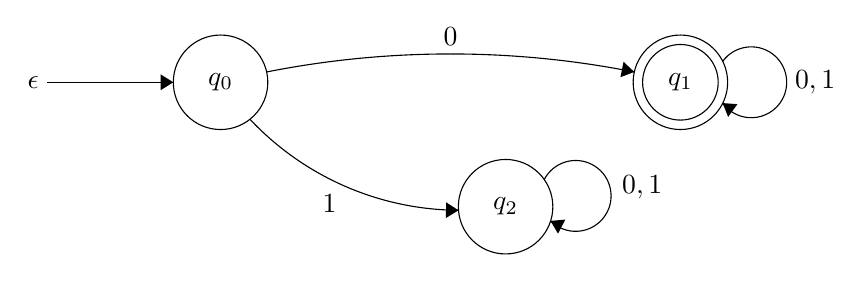
\begin{tikzpicture}[scale=0.2]
	\tikzstyle{every node}+=[inner sep=0pt]
	\draw [black] (20.6,-27.7) circle (3);
	\draw (20.6,-27.7) node {$q_0$};
	\draw [black] (49.8,-27.7) circle (3);
	\draw (49.8,-27.7) node {$q_1$};
	\draw [black] (49.8,-27.7) circle (2.4);
	\draw [black] (38.7,-35.6) circle (3);
	\draw (38.7,-35.6) node {$q_2$};
	\draw [black] (23.527,-27.044) arc (101.19936:78.80064:60.1);
	\fill [black] (46.87,-27.04) -- (46.19,-26.4) -- (45.99,-27.38);
	\draw (35.2,-25.4) node [above] {$0$};
	\draw [black] (52.48,-26.377) arc (144:-144:2.25);
	\draw (57.05,-27.7) node [right] {$0,1$};
	\fill [black] (52.48,-29.02) -- (52.83,-29.9) -- (53.42,-29.09);
	\draw [black] (35.712,-35.827) arc (-90.34893:-136.81015:18.322);
	\fill [black] (35.71,-35.83) -- (34.92,-35.32) -- (34.91,-36.32);
	\draw (27.52,-34.81) node [below] {$1$};
	\draw [black] (41.148,-33.885) arc (152.74451:-135.25549:2.25);
	\draw (46.07,-34.38) node [right] {$0,1$};
	\fill [black] (41.55,-36.5) -- (42.03,-37.31) -- (42.49,-36.42);
	\draw [black] (9.6,-27.7) -- (17.6,-27.7);
	\draw (9.1,-27.7) node [left] {$\epsilon$};
	\fill [black] (17.6,-27.7) -- (16.8,-27.2) -- (16.8,-28.2);
	\end{tikzpicture}
\end{center}



Un autómata puede presentarse también a modo de grafo como vemos, los estados se representan como nodos y los arcos representan las transiciones que modela la función $\delta(\cdot)$. Es decir, leemos la palabra de izquierda a derecha y por cada símbolo de la palabra, buscamos cuál es la transición asociada al estado en que nos encontramos y el símbolo que estamos leyendo.

\vspace{10px}

Ahora bien, uno de los estados está marcado con dos circunferencias, este es un estado final, al ser el único: $F = \{q_1\}$. El resto de los elementos de la tupla serían:

\begin{multicols}{2}
	\begin{itemize}
		\item $Q =\{q_0,q_1,q_2\}$
		\item $\mathcal{A} = \{0,1\}$
		\item $F = \{q_1\}$
	\end{itemize}
	
\end{multicols}

En cuanto a la función de transición, tendremos que el par $(a,q_i)$ pertenece al dominio de la función, si en el grafo existe un arco que salga de $q_i$ con etiqueta $a$. Las transiciones serían las siguientes:

\begin{multicols}{2}
	\begin{itemize}
		\item $\delta(0,q_0)=q_1$
		\item $\delta(1,q_0)=q_2$
		\item $\delta(a,q_1)=q_1 \ \forall a \in \{0,1\}$
		\item $\delta(a,q_2)=q_2 \ \forall a \in \{0,1\}$
	\end{itemize}
\end{multicols}

El símbolo $\epsilon$ se reserva para la palabra vacía, que es una entelequia que simboliza la palabra que no contiene ninguna letra.





\subsubsection{No-Determinismo}

Los autómatas que hemos examinado antes son deterministas, es decir, dada una entrada y partiendo de un estado, es trivial averiguar en qué estado acabaremos una vez leída esta. Sin embargo podemos considerar qué pasaría si nuestra función define las siguientes transiciones:

\begin{multicols}{2}
	\begin{itemize}
		\item $\delta(0,q_i)=q_j$
		\item $\delta(0,q_i)=q_k \hspace{2cm} j\neq k$
	\end{itemize}
\end{multicols}


Es decir: ¿Qué hacemos si estando el estado $q_i$ leemos un $0$? ¿Nos vamos a $q_j$ o a $q_k$? La respuesta no es simple. Los autómatas finitos no deterministas nacen por su enorme capacidad de expresión y su definición menos rigurosa que la de los anteriores. Sería una gran ventaja que fuesen equivalente, de manera que pudiésemos usar este último, más sencillo de definir, y aun así tener la potencia expresiva del anterior. La respuesta será que sí. 

\vspace{10px}


Su definición es parecida a la anterior salvo por un detalle, la función de transición:

\vspace{0.20cm}

$$\delta :Q\times \mathcal{A} \rightarrow \mathcal{P}(Q)$$

\vspace{0.3cm}

Aquí $\mathcal{P}(Q)$ es el conjunto potencia de $Q$, las partes de $Q$, es decir, dado un estado y un símbolo, podemos construir un autómata que tenga una arco conectando este estado $q_i$ con todos los demás incluyendo el mismo.



\newpage

Supongamos el siguiente problema, queremos crear un autómata que nos distinga  si una palabra pertenece a este lenguaje:

$$\{ \omega \in \{0,1\}^* : \omega \text{ tiene un número par de 0's} \} \cup \{\omega  \in \{0,1\}^*: \omega \text{ contiene al cadena }  101 \}$$

\begin{center}
	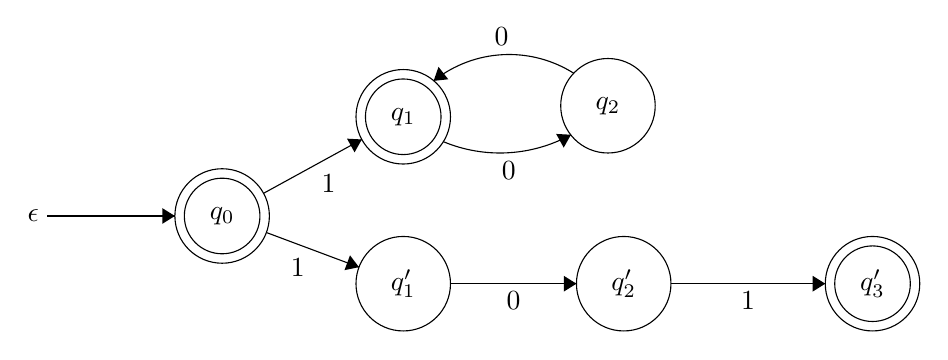
\begin{tikzpicture}[scale=0.2]
	\tikzstyle{every node}+=[inner sep=0pt]
	\draw [black] (17.2,-29) circle (3);
	\draw (17.2,-29) node {$q_0$};
	\draw [black] (17.2,-29) circle (2.4);
	\draw [black] (28.7,-22.7) circle (3);
	\draw (28.7,-22.7) node {$q_1$};
	\draw [black] (28.7,-22.7) circle (2.4);
	\draw [black] (28.7,-33.3) circle (3);
	\draw (28.7,-33.3) node {$q_1'$};
	\draw [black] (41.7,-22) circle (3);
	\draw (41.7,-22) node {$q_2$};
	\draw [black] (42.7,-33.3) circle (3);
	\draw (42.7,-33.3) node {$q_2'$};
	\draw [black] (58.5,-33.3) circle (3);
	\draw (58.5,-33.3) node {$q_3'$};
	\draw [black] (58.5,-33.3) circle (2.4);
	\draw [black] (6.1,-29) -- (14.2,-29);
	\draw (5.6,-29) node [left] {$\epsilon$};
	\fill [black] (14.2,-29) -- (13.4,-28.5) -- (13.4,-29.5);
	\draw [black] (19.83,-27.56) -- (26.07,-24.14);
	\fill [black] (26.07,-24.14) -- (25.13,-24.09) -- (25.61,-24.96);
	\draw (23.95,-26.35) node [below] {$1$};
	\draw [black] (20.01,-30.05) -- (25.89,-32.25);
	\fill [black] (25.89,-32.25) -- (25.32,-31.5) -- (24.97,-32.44);
	\draw (22.01,-31.67) node [below] {$1$};
	\draw [black] (39.348,-23.841) arc (-61.15181:-112.68383:9.343);
	\fill [black] (39.35,-23.84) -- (38.41,-23.79) -- (38.89,-24.66);
	\draw (35.4,-25.54) node [below] {$0$};
	\draw [black] (31.7,-33.3) -- (39.7,-33.3);
	\fill [black] (39.7,-33.3) -- (38.9,-32.8) -- (38.9,-33.8);
	\draw (35.7,-33.8) node [below] {$0$};
	\draw [black] (45.7,-33.3) -- (55.5,-33.3);
	\fill [black] (55.5,-33.3) -- (54.7,-32.8) -- (54.7,-33.8);
	\draw (50.6,-33.8) node [below] {$1$};
	\draw [black] (30.625,-20.424) arc (128.5933:57.57106:7.686);
	\fill [black] (30.63,-20.42) -- (31.56,-20.32) -- (30.94,-19.53);
	\draw (34.95,-18.21) node [above] {$0$};
	\end{tikzpicture}
\end{center}

Si nos fijamos, los estados $q_i'$ y los $q_i'$ conforman 2 autómatas independientes, que hemos unido usando el no-determinismo en la transición $\delta(q_0,1)$ hemos dado un autómata que reconoce únicamente las palabras del lenguaje unión, uniendo los autómatas.

\vspace{10px}

Esto se puede extender todavía más, introduciendo el concepto de las transiciones nulas. Una transición nula es la manera más cómoda de unir dos autómatas pues puedes moverte por libertad por todos los estados entre los que haya una transición nula. Intuitivamente esto quiere decir que podemos ir de un estado a otro sin leer el símbolo actual. 


\subsubsection{Ejemplos de Autómatas}

Después de estas consideraciones, queda pensar cuál es el papel de estos modelos en cuanto a su papel en temas de robótica. Pues pensemos en una función relativamente simple que querríamos que tuviese un robot, la comunicación por ejemplo.

\vspace{10px}

Un protocolo de comunicación es de los requerimientos más fundamentales, ya no en la robótica sino en cualquier sistema de relativa complejidad pues la función en sí es tan importante como la existencia de una interfaz de comunicación con el beneficiario de la función a implementar. No nos referimos necesariamente a la capacidad de expresión del agente, sino a la existencia de un protocolo que le permita transmitir información de forma coherente y exacta con el humano con el que interaccione, aunque este sea su programador.

\vspace{10px}

Hablamos por ejemplo de la implementación del protocolo TCP/IP, que en el fondo, es una máquina de estados finita o como lo venimos llamando: un autómata finito determinista. Daremos un ejemplo de cómo modelar un sistema de autenticación de usuarios con una máquina de estados muy simple.

\begin{itemize}
	\item $q_0$ Estado Inicial: En espera
	\item $F=\{q_1\}$ Único estado final : Autentificado
	\item $\mathcal{A}=\{001,010,011,000\}$
\end{itemize}

En cuanto a la función de transición. Supongamos que nuestro sistema incorpora la siguiente directivas:

\begin{multicols}{2}
	\begin{itemize}
		\item Envío de contraseña incorrecta: $001$
		\item Envío de contraseña correcta: $010$
		\item Salir: $011$
		\item Error: $000$
	\end{itemize}
\end{multicols}

\vspace{1cm}

\begin{center}
	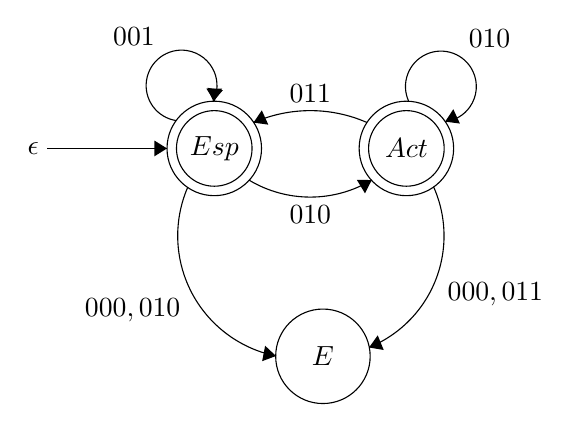
\begin{tikzpicture}[scale=0.2]
	\tikzstyle{every node}+=[inner sep=0pt]
	\draw [black] (37,-18.6) circle (3);
	\draw (37,-18.6) node {$Esp$};
	\draw [black] (37,-18.6) circle (2.4);
	\draw [black] (49.2,-18.6) circle (3);
	\draw (49.2,-18.6) node {$Act$};
	\draw [black] (49.2,-18.6) circle (2.4);
	\draw [black] (43.9,-31.8) circle (3);
	\draw (43.9,-31.8) node {$E$};
	\draw [black] (39.494,-16.958) arc (113.75402:66.24598:8.952);
	\fill [black] (39.49,-16.96) -- (40.43,-17.09) -- (40.02,-16.18);
	\draw (43.1,-15.7) node [above] {$011$};
	\draw [black] (46.998,-20.609) arc (-58.98762:-121.01238:7.566);
	\fill [black] (47,-20.61) -- (46.05,-20.59) -- (46.57,-21.45);
	\draw (43.1,-22.19) node [below] {$010$};
	\draw [black] (37,-15.5) -- (37,-15.6);
	\fill [black] (37,-15.6) -- (37.5,-14.8) -- (36.5,-14.8);
	\draw [black] (34.59,-16.833) arc (261.47443:-26.52557:2.25);
	\draw (31.9,-12.1) node [above] {$001$};
	\fill [black] (36.94,-15.61) -- (37.55,-14.9) -- (36.56,-14.75);
	\draw [black] (26.4,-18.6) -- (34,-18.6);
	\draw (25.9,-18.6) node [left] {$\epsilon$};
	\fill [black] (34,-18.6) -- (33.2,-18.1) -- (33.2,-19.1);
	\draw [black] (50.924,-21.032) arc (24.0977:-67.85012:7.646);
	\fill [black] (46.83,-31.24) -- (47.76,-31.4) -- (47.38,-30.47);
	\draw (51.79,-27.89) node [right] {${000,011}$};
	\draw [black] (40.919,-31.779) arc (-101.43921:-203.36619:7.786);
	\fill [black] (40.92,-31.78) -- (40.23,-31.13) -- (40.04,-32.11);
	\draw (34.88,-28.9) node [left] {${000,010}$};
	\draw [black] (49.35,-15.615) arc (204.86229:-83.13771:2.25);
	\draw (54.48,-12.2) node [above] {$010$};
	\fill [black] (51.66,-16.9) -- (52.6,-17.02) -- (52.18,-16.11);
	\end{tikzpicture}
\end{center}


Podríamos codificar los estados de $Esp$ (espera) y $Act$ (activo) como $000$ y $100$ con lo que tendríamos el estado de error ($E$) codificado como $101$. El autómata describe los posibles pasos en la autenticación de un usuario en un sistema, los estados de 'espera' y 'activo' serían finales dado que son estados 'correctos' en un posible sistema como este. El estado de error, describe justo eso, un comando que no se esperaba dado el estado de la comunicación en el que estábamos. Con este modelo podríamos construir un sistema de autenticación de usuarios usando 3 bits únicamente.


\subsection{La jerarquía de Chomsky}

El lenguaje que puede reconocer un autómata finito recibe el nombre de lenguaje regular, ya sea el autómata determinista, no-determinista o no-determinista con transiciones nulas, pues como comentábamos el paso de uno a otro se lleva a cabo mediante un procedimiento algorítmico. 

\vspace{10px}

Un concepto íntimamente relacionado con el de lenguaje, como aquí lo hemos visto, es el concepto de gramática, a saber: las reglas de producción a seguir para crear una palabra del lenguaje. Distinguiremos símbolos terminales (escritos con letras mayúsculas) y símbolos no-terminales, notados con letras minúsculas. La gramática asociada a un lenguaje regular tiene la siguiente forma:


$$ A \rightarrow a B \quad \quad A \rightarrow a$$ 

Esto quiere decir que cada símbolo no terminal se intercambia por un símbolo terminal y otro no terminal a lo sumo y que, cada símbolo no terminal es resoluble, es decir, siempre se puede intercambiar por uno terminal. Pongamos un ejemplo: 

\vspace{10px}

Sea $\mathcal{L}=\{0,1\}^*$ el conjunto de todas las palabras que se pueden formar yuxtaponiendo 0's y 1's. Su gramática vendría dada por:


\begin{multicols}{2}
	\begin{itemize}
		\item $A \rightarrow 1$
		\item $A \rightarrow 0$
		\item $A \rightarrow 1A$
		\item $A \rightarrow 0A$  
	\end{itemize}
\end{multicols}


Esta gramática es muy sencilla debido al alto número de restricciones bajo las que se ha concebido, si eliminamos dichas restricciones aumentamos la expresividad del lenguaje, aumentando así la complejidad del modelo de computación que tendrá asociado, como el caso de los autómatas finitos para los lenguajes regulares.

\vspace{10px}

Pues bien, la jerarquía de Chomsky es una estructura piramidal que refleja cómo aumenta la complejidad del lenguaje conforme eliminamos restricciones en la gramática:

\vspace{1cm}


\begin{center}
	\begin{tabular}{|c|c|c|c|}
		\hline 
		Gramática & Lenguaje  &Reglas de producción   & Autómata  \\ 
		\hline 
		Tipo 0	& recursivamente enumerable  & sin restricciones  & Máquina de Turing  \\ 
		\hline 
		Tipo 1	& dependiente del contexto  & $\alpha A \beta \rightarrow \alpha \gamma \beta$ & linealmente acotado  \\ 
		\hline 
		Tipo 2	& independiente del contexto  & $A \rightarrow \gamma $  & autómata con pila   \\ 
		\hline 
		Tipo 3	& regular  & (*) & autómata finito \\
		\hline 
	\end{tabular} 
\end{center}

\vspace{1cm}

Los autómatas con pila presentan una generalización de los autómatas finitos. Ya no tenemos una representación tipo grafo pero la manera de leer símbolos con la función $\delta(\cdot)$ es similar. Resaltamos que además del criterio de estados finales ( si terminamos de leer una palabra y estamos en un estado final la palabra es aceptada) los autómatas con pilas presentan un criterio de aceptación equivalente: el criterio de pila vacía; es decir: si al terminar de leer la palabra la pila del autómata está vacía se considerará una palabra válida. Esto se debe a que al leer un símbolo en la palabra en este tipo de autómatas podemos meter o sacar símbolos específicos de una pila ( LIFO ).

\vspace{10px}

Sin embargo, daremos un salto cualitativo importante e iremos directamente al modelo computacional más complejo de la jerarquía: Las Máquinas de Turing.



\subsection{La Máquina de Turing}

 Una Máquina de Turing es un tipo de autómata con memoria infinita, se dispone de un conjunto de cardinal numerable infinito en el que podemos guardar símbolos e información temporal. La manera más sencilla de pensar en dichas máquinas es como una pareja: un cabezal lector y una cinta infinita. El cabezal lee un símbolo y se mueve a izquierda o a derecha dependiendo de la función de transición, de manera rigurosa, una Máquina de Turing es una séptupla $MT=(Q,A,B,\delta,q_0,\#,F)$


\begin{multicols}{2}
	\begin{itemize}
		\item $Q$  Conjunto finito de estados
		\item $A$  Alfabeto de entrada
		\item $B$  Alfabeto de símbolos en la cinta , $A\subset B$
		\item $\delta$ Función de transición
		\item $q_0$ Estado inicial
		\item $\# \in B-A$ El 'símbolo blanco'	
		\item $F$ Conjunto de estados finales 
	\end{itemize}
\end{multicols} 
 
 
 Una transición típica de una Máquina de Turing sería: $\delta(q_0,0)=(q_1,\#,D)$. Esto quiere decir que si estando en el estado $q_0$ el cabezal lector de la cinta está posicionado sobre una de las celdas de la cinta que contiene un 0, cambiaremos dicho 0 por un $\#$ y moveremos el cabezal lector a la derecha.
 
 \vspace{10px}
 
 A diferencia de un autómata finito que tenía que leer la palabra entera para verificar que pertenecía al lenguaje, se dice que una Máquina de Turing acepta una palabra siempre y cuando llegue a un estado de aceptación, aunque queden símbolos por leer.
 
 \vspace{10px}
 
 En caso de que lleguemos a un estado no final y ya hayamos terminado de leer la palabra se dice que esta se ha rechazado; el problema llega cuando la máquina cicla de manera indefinida.


\subsubsection{El problema de la parada}


Acabamos de mencionar el problema que se presenta cuando una Máquina de Turing no para, pues aunque técnicamente no rechaza la palabra tampoco la acepta. Existe una equivalencia entre función computable ( algoritmo ) y Máquina de Turing (\textbf{Tesis de Church-Turing}), entonces: dada una entrada para un algoritmo o de manera equivalente, dada una máquina de Turing y una palabra sobre su alfabeto ¿Es posible saber si la palabra será aceptada o rechazada? La respuesta es que no.

\vspace{10px}

Alan Turing en su artículo \textbf{On Computable Numbers, with an Application to the Entscheidungsproblem} (1936) demostró que existían problemas indecidibles, entre los cuales se encuentra este. La demostración es sencilla:

\vspace{10px}

Supongamos que existe $Stop(P,x)$ un algoritmo capaz de averiguar si el programa $P$ para con los datos $x$. Construimos entonces:

\begin{lstlisting}
Turing(P):

L	If Stops(P,P), GOTO L
\end{lstlisting}

\vspace{0.5cm}

Al considerar $Turing(Turing)$ llegamos a contradicción pues el programa para si y solo si no para.

%TODO http://mathworld.wolfram.com/UniversalTuringMachine.html
\subsubsection{Máquinas de Turing Universales}

Las Máquinas de Turing pueden codificarse mediante símbolos, una Máquina de Turing capaz de leer una codificación de este tipo y comportarse como dicha máquina se conoce como Máquina Universal de Turing. Un sistema de cómputo que pueda comportarse de esta manera se dice Turing-completo.

\vspace{10px}

La primera máquina Turing-completa fue el Z3 de Zuse construida en 1941, aunque dicha propiedad fuese demostrada por Raúl Rojas en 1998.

\vspace{10px}

Este es uno de los saltos cualitativos de mayor relevancia en la historia de la computación pues es el inicio de los ordenadores tal y como los conocemos, máquinas capaces de leer algoritmos y ejecutarlos, capaces de ser cualquier máquina.

\vspace{10px}

Aunque \textit{a priori} parezca una propiedad muy complicada de tener veremos que existen numerosos sistemas que poseen esta propiedad, no sólo modelos teóricos tremendamente complejos, existen una sería de sistemas, en su mayoría juegos, que poseen esta propiedad, quizá el más señalado sea el juego de la vida de Conway. Aunque también podemos contar al 'Pokemon Amarillo' entre los elegidos.

%http://aurellem.org/vba-clojure/html/total-control.html



%TODO meter cita
\subsubsection{El juego de la vida: casualmente Turing-completo}

El juego de la vida consta de un tablero, en él, las celdas pueden clasificarse como vivas o muertas, se pintan en negro o blanco dependiendo de en qué categoría se encuentren. Una configuración inicial sería un conjunto cualquiera de células vivas. El juego posee 2 reglas:

\begin{multicols}{2}
	\begin{itemize}
		\item Una casilla con exactamente 3 vecinas 'vivas' nace.
		\item Una casilla con 2 o 3 vecinas vivas sigue viva, en otro caso muere.
	\end{itemize}
\end{multicols}


Pues bien, este juego de 0 jugadores, con estas dos reglas es Turing-completo.

%TODO citar el libro de paco
\subsection{Inteligencia Artificial}

Abordaremos ahora cómo ha ido evolucionando el paradigma de la inteligencia artificial, desde la inteligencia fuerte ( hacer que las máquinas sean inteligentes ) hasta la débil (hacer que se comporten de manera inteligente).

\vspace{10px}


El término 'inteligencia artificial' se acuñó en el año 1955 en la 'Conferencia de Dartmouth' y describía la inteligencia artificial como : 'la ciencia e ingeniería de hacer máquinas que se comporten de una forma que llamaríamos inteligente si un humano tuviese dicho comportamiento'.

\vspace{10px} 

Como campo de investigación nace un año después en 1956, en la ciudad de Hannover,New Hampshire (EEUU). Mencionaremos otras dos definiciones que muestran la dualidad de la que hablábamos antes:

\begin{itemize}
	\item 'La inteligencia artificial está relacionada con conductas inteligentes en artefactos' (Nilsson,1998).
	\item 'El nuevo y excitante esfuerzo de hacer que los computadores piensen...,máquinas con mentes, en el sentido más literal' (Haugeland,1985).
\end{itemize}

La primera definición se centra más en lo que hemos llamado 'inteligencia débil': conseguir que una máquina se comporte de manera inteligente. La segunda es algo más problemática pues si nos cuesta definir y entender el concepto de inteligencia, dotar a un ser inanimado de capacidad de pensamiento como tal, se plantea como un problema mucho más complicado que cualquiera con el que nos hayamos topado antes.

\vspace{10px}

A colación de esto último comentamos que Turing escribió un articulo en 1950 llamado 'Computing machines and intelligence' en el que propone cuestiones como: ¿Pueden pensar las máquinas?


\subsubsection{El Test de Turing}

En dicho artículo Turing propuso un 'test', una prueba que podría hacérsele a una computadora para comprobar si en efecto, presenta algún tipo de inteligencia.

\vspace{10px}

En dicha prueba una persona conversa con un interlocutor al que no ve e intenta adivinar si dicho interlocutor es un ser humano o una computadora. Si la computadora consigue engañar al humano se dice que ha pasado el test. Evidentemente esta conversación no puede delimitarse a ningún tema trivial o a un campo muy delimitado, donde sería fácil engañar al interlocutor humano.

\vspace{10px}

Destacamos la siguiente noticia del diario \href{https://www.abc.es/ciencia/20140609/abci-superordenador-supera-primera-test-201406091139.html}{\textbf{ABC}} de 2014 en el que un ordenador fue capaz de engañar a los jueces del test, haciéndoles creer que era un joven ucraniano de 13 años.


\subsubsection{La habitación china}

El test de Turing puede parecer a primera vista un método que, bajo una prueba suficientemente rigurosa, puede aportar un aserto creíble en torno a si la máquina en cuestión está teniendo un comportamiento inteligente; es decir: es capaz de engañar a su interlocutor humano captando y entendiendo el significado de los mensajes y respondiendo de manera acorde. Sin embargo existen críticas a este test, la más famosa, \textbf{la habitación china}: Este experimento modela una situación en el que se pasaría el test de Turing sin haber demostrado ningún comportamiento inteligente, invalidando el test.

Supongamos que tenemos la siguiente disposición en la prueba del test de Turing. Tenemos dos interlocutores, uno comunicándose en chino y otro en inglés. De manera que el interlocutor inglés tiene en su poder una chuleta para el examen, un conjunto de reglas que especifican cuál es la respuesta, de manera detallada, para los caracteres de entrada. Entonces, podría existir una comunicación real entre los dos interlocutores sin que uno de ellos tuviese idea alguna del contenido de los mensajes.

\vspace{10px}

El interlocutor inglés pasaría la prueba del test de Turing burlando su metodología, sin haber demostrado un comportamiento inteligente, emparejando únicamente respuestas y preguntas sin llegar a comprender nada de su contenido.

\vspace{10px}

El problema reside en que definir qué es ser inteligente es complicado, pues como comentamos al principio del texto, hay numeroso grupos de elementos en este campo que clasificamos por extensión. Un comportamiento es inteligente si es parecido a un comportamiento que ya teníamos categorizado como inteligente. El espíritu del test de Turing refleja esto a la perfección pues concluimos que la máquina es inteligente si es capaz de reproducir un comportamiento humano que ya hemos concluido que es inteligente. 

\vspace{10px}

Sin embargo, al igual que planteamos con el concepto de 'máquina' al principio, se hace complicado saber de manera concisa y concreta si un elemento pertenece a un grupo generado por extensión, clara prueba de ello es \textbf{la habitación china} que, teóricamente, invalida el test de Turing, que aun con todo esto, sigue en uso.

\subsubsection{Agentes Inteligentes}


La noción de agente es parecida a la definición de autómata más clásica: un sistema capaz de interactuar de forma automática con el entorno, dotado de sensores y con capacidad de reaccionar ante la información que estos le brinden. La clase de complejidad a la que pertenezcan estos agentes ya es harina de otro costal; podríamos tener un ordenador (Máquina de Turing universal), controlando un agente, con lo cual su modelo de complejidad teórico estaría en lo alto de la jerarquía. También podríamos tener un agente con un mecanismo de respuesta muy sencillo descrito por un autómata, lo mostramos con un ejemplo.


\vspace{10px}

Quizá la manera más familiar de pensar en un agente es imaginarlo como un robot de limpieza. Tenemos un mecanismo, capaz de llevar a cabo una tarea de forma automática, basándose en la información que percibe de unos sensores y en alguna forma programada de toma de decisiones. Dependiendo de lo laboriosa que sea el mecanismo de toma de decisiones, el agente podrá ser clasificado en uno de los campos de complejidad que comentábamos antes; pero sea cual sea, categoriza como agente.

\vspace{10px}

Supongamos que uno de estos agentes tiene el siguiente mecanismo de toma de decisiones. El agente puede estar en movimiento o haber chocado, en caso de haber chocado giramos de manera aleatoria a izquierda o a derecha 90º y seguimos recto. Bueno, por muy sencillo que sea este funcionamiento, el robot se moverá y limpiará la habitación ( aunque es posible que se quede dando vueltas en alguna esquina ). Esto se conoce como \textbf{agente reactivo}: un agente que toma decisiones basándose únicamente en los input actuales. Estos agentes se encontrarían en la escala de complejidad más baja, son \textbf{sistemas combinacionales}, pues no guardan información anterior para orientarse y tienen predefinida una respuesta para los estímulos de entrada producidos por los sensores.


\vspace{10px}

Podemos pensar que tener tantos modelos de computación para crear un robot como el que acabamos de describir es decepcionante. Pues de aquí nace el concepto de \textbf{agente deliberativo}. Es decir, el agente no solo reacciona al impulso, delibera sobre el input e intenta tomar la 'mejor opción'. Un agente se considera deliberativo cuando tiene en memoria un esquema de representación del mundo en el que se mueve. Una vez más vemos como la capacidad de tener memoria nos permite dar saltos cualitativos en lo que a complejidad se refiere.

\vspace{10px}

En contraposición al primer ejemplo, supongamos de nuevo que el agente ha chocado; este sería un típico comportamiento deliberativo: Marcar en memoria que en la posición actual hay un muro, planificar una ruta (usando el algoritmo $A^*$ por ejemplo) a la siguiente zona por la que no hayamos pasado todavía y seguir recorriendo la habitación.

\subsubsection{Las tortugas de Walter: un ejemplo de agente}

Estos agentes fueron diseñados en 1948 por W. Grey Walter, cuya intención era la de probar que con mecanismos rudimentarios se podían crear comportamientos complejos. La funcionalidad básica del robot era la siguiente: constaban de 2 grupos de sensores unos de presión para evitar choques y otros fotosensibles. Además los robots podían moverse y girar con libertad y autonomía.

\vspace{10px}

Los robots levantaron bastante expectación pues estaban programados para acercarse o alejarse de la luz dependiendo de el estado de su batería. Esto coincidía con el hecho de que las plataformas de carga se situasen cercanas a los focos de luz intensa. Estos agentes conseguían moverse con cierta libertad y mostraban comportamientos típicos de animales, acercarse o alejarse de la luz dependiendo de su ciclo 'energético'; pero, ¿Es esto un comportamiento inteligente?

\vspace{10px}

Aunque es verdad que siguiendo la definición purista hay que considerarlos como agentes deliberativos, pues toman la acción de acercarse o alejarse de la luz en función de unos parámetros de representación interna (como es el porcentaje de carga en este caso),presentan un comportamiento y un razonamiento bastante limitado en comparación con algo con lo que podemos estar muy acostumbrados: un típico robot de limpieza, como comentábamos antes.

\subsection{Fronteras}

Por último queremos destacar la delgada linea que encontramos entre muchos de los conceptos de los que hemos hablado. Es decir: los extremos están controlados, queda claro que \textbf{Deep Blue} (1996), presentaba un comportamiento inteligente; también queda claro que una tostadora (por muy útil que sea) no lo presenta; pero, ¿Qué pasa si empezamos a añadirle funcionalidades a la tostadora? Si por ejemplo fuese capaz de saber cuando las tostadas están hechas y nunca las quemase ya entraría en consideración como agente reactivo. Las siguientes preguntas quedan sin responder: ¿Cómo de inteligente es un comportamiento dado?, ¿A partir de qué momento sería la tostadora inteligente?, ¿Queda mucho para vivir en el utópico mundo en el que no haya que rascar 'lo quemado' de las tostadas?

\vspace{10px}

Estas preguntas son más serias de lo que parecen en un mundo cada vez más informatizado. Desde luego llamamos inteligentes a los móviles, son MTU claramente, un concepto alejado de la implementación del protocolo de comunicación que supusieron en un principio.. 

\vspace{10px}

Citando a Turing (1950): \textbf{'Solo podemos prever el futuro inmediato, pero de lo que cabe duda es de que hay mucho por hacer'}.



\newpage
	
